\documentclass[11pt,onecolumn]{article}
\usepackage[a4paper, top=2.6cm, bottom=2.4cm, left=3.1cm, right=3.1cm]{geometry}
\usepackage[T1]{fontenc}
\usepackage[utf8]{inputenc}
\usepackage{amsfonts}
%\usepackage[style=long]{glossaries}
\usepackage{hyperref}
\usepackage{amsthm}
\usepackage{fancyhdr}
\usepackage{amsmath}
\usepackage{wasysym}
\usepackage{enumerate}
\usepackage{multicol}
\usepackage{units}
\usepackage{cancel}
\usepackage{graphicx}
\usepackage{psfrag}
\usepackage{verbatim}
\usepackage{subfigure}
\usepackage{amssymb,amsmath,amsbsy}
\usepackage{textcomp}
\usepackage{graphicx}
\usepackage{mathtools}
\usepackage{float}
\usepackage{pdfpages}
\usepackage[font=small,format=plain,labelfont=bf,up,textfont=it,up]{caption}
\usepackage{parskip}
\usepackage{booktabs}
\usepackage{xcolor}
\usepackage{listings}

\newcommand{\sect}[1]{Section~\ref{#1}}
\newcommand{\fig}[1]{Figure~\ref{#1}}
\newcommand{\eq}[1]{(\ref{#1})}

\newcommand{\showcodeappendix}[1]{
\lstinputlisting[breaklines=true,captionpos=b,language=Erlang,showlines=true,
basicstyle=\ttfamily\footnotesize]{#1}}

\newcommand{\showcodebox}[1]{
\lstinputlisting[breaklines=true,captionpos=b,frame=tblr,showlines=true,
language=Erlang,basicstyle=\ttfamily\small]{#1}}

\newcommand{\showcodeboxwithlabel}[2]{
\lstinputlisting[breaklines=true,captionpos=b,frame=tblr,showlines=true,
label={#1},language=Erlang,basicstyle=\ttfamily\small]{#2}}

\newcommand{\showcodehalfbox}[1]{
\lstinputlisting[breaklines=true,captionpos=b,frame=tbl,showlines=true,
language=Erlang,basicstyle=\ttfamily\small]{#1}}

\newcommand{\showcodehalfboxwithlabel}[2]{
\lstinputlisting[breaklines=true,captionpos=b,frame=tbl,showlines=true,
label={#1},language=Erlang,basicstyle=\ttfamily\small]{#2}}


% Bibliography
%\usepackage[citestyle=numeric-comp, sorting=none]{biblatex}
%\bibliography{include/references}
%\renewcommand{\bibfont}{\normalfont\small}

% Horizontal rule command for title page
\newcommand{\HRule}{\rule{\linewidth}{0.2mm}}

% Settings (Metadata)
% Number of deliverable
\newcommand{\cmdDlNumber} %
{D3.3}

% Name of deliverable
\newcommand{\cmdDlName} 
{Report on tools and techniques to model, in an uniform way, the differences between different versions of a system, 
which are parametrized or configured in different ways.}

% Number of work package
\newcommand{\cmdWpNumber}
{WP3}

% Name of work package
\newcommand{\cmdWpName}
{Dealing with multiplicity and evolution}

% Authors name(s)
\newcommand{\cmdNames}{%
	Ramsay Taylor (USFD)\\
	Pablo Lamela Seijas (KENT)\\
	John Derrick (USFD)\\
        Stephen Adams (KENT)\\
	Simon Thompson (KENT)
}

% Nature of deliverable (Prototype/Report/Other)
\newcommand{\cmdDlNature}
{Report}

% Contractual date of delivery (dd/mm/yy)
\newcommand{\cmdDlContractDate}
{30/09/15}

% Actual date of delivery (dd/mm/yy)
\newcommand{\cmdDlActualDate}
{30/09/15}

% Document ID
\newcommand{\cmdDlDocumentId}
{Prowess/2015/D3.3/v1.0}

% Dissemination (PU/PP/RE/CO)
\newcommand{\cmdDlDissemination}
{PU}

% Reviewer name
\newcommand{\cmdDlReviewerName}
{Thomas Arts}

% links to demos, source code, papers, etc
\newcommand{\cmdDlWeblinks}
{<links to demos, source code, papers, etc>}

% Keywords
\newcommand{\cmdDlKeywords}
{parametrisation, EFSM inference, behaviour extraction, erlang-diff}

% Abstract (Up to half a page describing the essential results contained in the deliverable)
\newcommand{\cmdDlAbstract}{%
This deliverable shows how the QuickCheck state-machine models, which are extended finite state 
machines (EFSMs), can be parametrised to support different configurations or versions of a system, and how
this task can be partially automated.
}

% PDF Metadata and link styles
\hypersetup{
	pdftitle={Deliverable \cmdDlNumber{} (\cmdWpNumber{})},%
	pdfauthor={PROWESS Project},%
	colorlinks=true,%
	citecolor=black,%
	filecolor=black,%
	linkcolor=black,%
	urlcolor=black
}


% Tighter itemize environment
\newenvironment{packed_itemize}{
\begin{itemize}
	\setlength{\itemsep}{1pt}
	\setlength{\parskip}{0pt}
	\setlength{\parsep}{0pt}
}{\end{itemize}}

% Tighter enumerate environment
\newenvironment{packed_enumerate}{
\begin{enumerate}
	\setlength{\itemsep}{1pt}
	\setlength{\parskip}{0pt}
	\setlength{\parsep}{0pt}
}{\end{enumerate}}

% Color for text colors in .doc template
\definecolor{prowessblue}{RGB}{0,51,102}
\definecolor{prowessred}{RGB}{128,0,0}

% Glossary
%\input{include/Glossary}

% Header and footer (defined in settings included above)
\cfoot{\thepage}
\lhead
{\small \cmdDlNumber{} / \cmdDlName{}} 
\rhead
{ \small  }
\renewcommand{\headrulewidth}{0pt} % Remove bar in header

\pagestyle{fancy}

\newcommand{\powerset}[0]{\mathbb P}

\def \bool  {{\mathbb B}}
\def \fun {\rightarrow}

\begin{document}

% Title page
% Beginning of titlepage
\begin{center}

\begin{flushright}
	FP7 Project ICT-2011-317820 PROWESS \\[-0.25cm]
\end{flushright}

\HRule \\[0cm]

\begin{flushright}
	PROWESS: Property Based Testing of Web services
\end{flushright}


\includegraphics[width=10cm]{figures/prowess_clr.png} \\[0.5cm]

{\large \color{prowessblue} \cmdDlNumber{} \cmdDlName{}} \\[-0.25cm]
\HRule \\[0cm]
{\color{prowessblue} \cmdNames{}}

\textbf{Abstract} \\
EU-ICT Specific targeted research project (STREP) ICT-2011-317820 \\
Deliverable \cmdDlNumber{} (\cmdWpNumber{})

\begin{flushleft}
	\cmdDlAbstract{}
\end{flushleft}

\HRule

\begin{flushleft}
	{\color{prowessblue} \textbf{Keyword list:} \cmdDlKeywords{}} \\[-0.1cm]
\end{flushleft}

\HRule

\begin{minipage}[t]{0.5\linewidth}
\begin{flushleft}
	\cmdWpNumber{} \cmdWpName{}\\
	Nature: {\color{prowessred} \cmdDlNature{}}\\
	Contractual date of delivery: {\color{prowessred} \cmdDlContractDate{}}\\
\end{flushleft}
\end{minipage}
\begin{minipage}[t]{0.49\linewidth}
	\begin{flushleft}
		Document ID: {\color{prowessred} \cmdDlDocumentId{}}\\
		Dissemination: {\color{prowessred} \cmdDlDissemination{}}\\
		Actual date of delivery: {\color{prowessred} \cmdDlActualDate{}}\\
	\end{flushleft}
\end{minipage}\\[0.3cm]
\begin{flushleft}
Reviewed by: {\color{prowessred} \cmdDlReviewerName{}}\\
%Weblinks: {\color{prowessred} \cmdDlWeblinks{}}
\end{flushleft}

\end{center}

\clearpage



% Consortium
% Consortium page
% Changes from .doc version: Wrote Torben with upper case T
\section*{PROWESS Consortium}
\addcontentsline{toc}{section}{Prowess Consortium}

This document is part of a research project partially funded by the IST Programme of the Commission of the European Communities as project number ICT-2011-317820.\\[0.2cm]

\begin{footnotesize}
% First column
\begin{minipage}[t]{0.5\linewidth}
	\textbf{University of Sheffield}\\
	Department of Computer Science\\
	Regent Court, 211 Portobello St.\\
	Sheffield S1 4DP\\
	UK\\
	Tel: +44 114 222 1930\\
	Fax: +44 114 222 1810\\
	Contact person: John Derrick\\
	E-mail: J.Derrick@dcs.shef.ac.uk\\
	\\
	
	\textbf{University of Canterbury}\\
	The Registry Canterbury,\\
	Canterbury,\\
	Kent, CT2 7NZ\\
	UK \\
	Tel: +44 1227 823820\\
	Fax: +44 1227 762811\\
	Contact person: Prof Simon Thompson\\
	E-mail: S.J.Thompson@kent.ac.uk\\
	\\
	
	\textbf{Chalmers Tekniska Hoegskola Aktiebolag}\\
	412 96\\
	Goteborg\\
	Sweden \\
	Tel: +46 707563760\\
	Contact person: Prof John Hughes\\
	E-mail rjmh@chalmers.se\\
	\\
	
	\textbf{Universidad Polit\'ecnica de Madrid}\\
	Dpto. LSIIS, Facultad de Informática, UPM.\\
	Campus de Montegancedo s/n, 28660 Boadilla\\
	del Monte, Spain\\
	Tel: +34 913366903\\
	Fax: +34  913363571\\
	Contact person: Lars-Ake Fredlund\\
	E-mail: lfredlund@fi.upm.es\\
	\\
	
	\textbf{Universidade da Coru\~na}\\
	Departamento de Computaci\'on (Lab 4.1)\\
	Facultade de Inform\'atica\\
	Campus de Elvi\~na S/N 15071 A Coru\~na\\
	Spain\\
	Tel: +34 981 167 000 ext. 1359\\
	Fax: +34 981 167 160\\
	Contact person: Dr. Laura M. Castro\\
	E-mail: lcastro@udc.es\\
\end{minipage}
% Second column
\begin{minipage}[t]{0.5\linewidth}
	\textbf{Quviq AB}\\
	Bergshamravagen 4\\
	433 60 Savedalen\\
	Sweden\\
	Tel: +46 70 4388567\\
	Contact Person: Thomas Arts\\
	Email Thomas.arts@quviq.com\\
	\\
	
	\textbf{Erlang Solutions LTD}\\
	New Loom House\\
	101 Back Church Lane\\
	London E1 1LU\\
    UK\\
	Tel: +44 2074561020\\
	Contact person: Torben Hoffmann\\
	E-mail: torben.hoffmann@erlang-solutions.com\\
	\\
	
	\textbf{Interoud Innovation SL}\\
	Avenida De  Alfonso Molina 53B\\
	15006 A Coruna\\
	Spain\\
	Tel: +34 981173344\\
	Contact person: Oscar Sacristan\\
	E-mail: oscar.sacristan@interoud.com\\
	\\
	
	\textbf{SP Sveriges Tekniska Forskningsinstitut AB}\\
	Brinellgatan 4\\
	501 15 Boras\\
	Sweden\\
	Tel: +46 105165359\\
	Contact person: Jonny Vinter\\
	E-mail: jonny.vinter@sp.se\\
\end{minipage}
\end{footnotesize}

\clearpage


% Executive summary
% Executive summary page
\section*{Executive Summary}
\addcontentsline{toc}{section}{Executive Summary}

This deliverable reports work from the revised task descriptions as contained in Deliverable D8.1.1. In particular, for Task 3.3 it makes the advance
\begin{quote}
In order to support large-scale configuration, and also system evolution, we will develop parametrised models and properties which can be used to produce tests for all the configurations, and which can be evolved as single artefacts rather than one configuration at a time. Support for these models and properties will be implemented as QuickCheck libraries, and a set of case studies will be develop to illustrate how parametric models can be built.
\end{quote}
Parametrised models are supported as Erlang behaviours, and these can be tested in exactly the same way as standard, non-parametric models. This solution, rather than Erlang parametrised models, was chosen for two reasons. First testing is supported in precisely the same way as for non-parametric models, and secondly parametrised modules are a deprecated feature of Erlang and support for them is likely to be removed in future releases of Erlang.

We have provided further support for parametric modelling by implementing facilities to
\begin{itemize}
\item
transform non-parametric models into parametric ones by providing refactoring support in Wrangler for an ``introduce behaviour'' refactoring, and its reverse, which unfolds a parametric model into a non-parametric model (Section \ref{sec:assisted-creation});
\item
provide decision support for parametrisation introduction by implementing a ``diff'' functionality for models, which will infer likely functionality for parametrisation from the difference of two Erlang modules (Section \ref{sec:identification});
\item
moreover, we have shown how these facilities work in practice in a set of case studies (Section \ref{sec:case-study}).
\end{itemize}



Extended Finite State Machines extend conventional Finite State Machines by incorporating a data state in addition to the control flow state of the standard machine. The transition labels are extended to incorporate guards that are boolean functions over the data space. The available transitions of the machine depend not only on its control flow state (as is the case for FSMs) but also on its data state, as some transitions may be prevented by their guards. Additionally, EFSM transition labels contain update transformations that modify the data state if the transition is executed. 

In using inference to find models of systems from the systems themselves, we have shown that finite state machine models can be inferred effectively, but in completing the work of Task 3.2 we show in Section \ref{EFSMInference} here that inference techniques can be extended to include machines with state data and conditional transitions. This is illustrated with a running example, and is the subject of a pilot study too.






\clearpage


\tableofcontents
\clearpage

\section{Introduction}

The Description of Work describes Task 3.3 thus
\begin{quote}
Task 3.3: Develop tools and techniques to model, in an uniform way, the differences between different versions of
a system, which are parametrized or configured in different ways.
\end{quote}

\subsection{Behaviour refactoring}

The abstraction principle tells us that we must not repeat code. As
stated by {[}citation{]} ``Each significant piece of functionality
in a program should be implemented in just one place in the source
code. Where similar functions are carried out by distinct pieces of
code, it is generally beneficial to combine them into one by abstracting
out the varying parts''. In practice we cannot always see what abstraction
we need until we have already replicated code. 

Having replicated code is bad because it forces us to make modifications
to the replicated code several times. We will eventually forget to
modify all the instances and we will go from having replicated code,
to having one subset of the bugs solved in one of the instances, and
another subset of them in the other one.

On the other hand, Erlang provides a mechanism for abstracting and
parametrising implementations at module level, this mechanism is Erlang
behaviours.

Erlang behaviours are composed of a behaviour definition and a number
of behaviour instances that implement the definition.
\begin{itemize}
\item The \emph{behaviour definition} is expected to contain the common
code, and provides an interface for the behaviour instances.
\item The \emph{behaviour instances} provide the particular implementations
and must implement the interface provided by the \emph{behaviour definition}.
\end{itemize}

\section{Related Work}
\label{related_work}

Diverse approaches and studies have been aimed in the past...

\section{Approach 1}
\label{approach1}

\section{Approach 2}
\label{approach2}

\section{Automatic creation of Erlang behaviours}

When developing software, we sometimes realise that we should add
abstraction after we have already implemented two pieces of similar
code. At this point, we must make an additional effort to find the
commonalities and unify them. This job is tedious and error prone,
and it does not provide any additional functionality, which makes
it difficult to justify. Nevertheless, it helps reduce maintenance
effort required in the future, and it will avoid the diversion in
the evolution of the code unified.

For this reason, in this section we study a mechanism that automatically
creates an Erlang behaviour by merging two modules selected by the
user, which are assumed to be structurally similar, and possibly the
result of copying and modifying one of them.

This mechanism has been implemented and distributed as a refactoring
included in Wrangler refactoring tool for Erlang {[}citation{]}, and
its source is available at {[}citation{]}. Even though there is no
guarantee about this, the refactoring aims to not alter the behaviour
of the two modules targeted from the point of view of their external
interface, and it should only affect the organisation of the code
between the original modules, (which will be transformed by the refactoring
into \emph{behaviour instances}), and the newly created \emph{behaviour
definition}.


\subsection{Related work}

Our approach has a lot in common with clone detection. The main difference
is that in this approach we assume that we know the root of the replication
and we are actually finding the different parts, and clone detection
assumes that most of the code is different and tries to find the commonalities.
In our case we assume that we start with two modules which are similar
and we try to find a common structure between both and create an Erlang
behaviour. For this reason the problem is not so much locating the
common parts but matching them appropriately. Thus, in our case it
makes more sense to explore structural commonalities in depth, whereas
in clone detection it is often more effective to focus on the sequential
behaviour.

The previous work that we have found which is most similar to the
one presented here is the ladiff tool {[}citation{]}, which strongly
inspired this work. Tree comparison has been researched extensively
{[}citations{]}, a big part targeted at XML {[}citation{]}. Of course,
the nature of XML is quite different to the one of Erlang, but they
both share the use of nested structures and semi-structured data.


\subsection{Overview}

The algorithm consists of three parts, tree matching, cluster construction,
and cluster linking. The process starts with two modules which are
assumed to be similar. First we find commonalities between their ASTs,
group the contiguous commonalities, move the commonalities to a separate
module, and link the pieces together with function calls in order
to preserve the original behaviour. This way we are left we three
modules, the remainings of the original ones and a new module with
the common parts.


\subsection{Tree matching\label{sub:tree-matching}}

In the first stage we apply a tree matching algorithm to find correspondences
between the ASTs, of both modules. In the current implementation we
have used the top-down tree matching algorithm described in {[}citation{]},
because it is both easy to implement and effective. But we have encapsulated
the tree matching algorithm in a way that would allow it to be replaced
easily by other algorithms in the future.

In particular, we have found some more recent and heavily tuned algorithms
that might work better for our approach, but we have discarded them
for this work because, due to their complexity, reimplementing them
would have been much more costly, and in the cases where there exist
public implementations of them, they are written in different languages,
(usually Java), which would have made the integration more difficult
and cumbersome.

The only consideration for applying tree matching to our problem is
deciding how to compare individual nodes of the syntax tree. We use
a simple dual approach:
\begin{itemize}
\item For leave nodes, which usually contain the semantic information, we
compare the literal representation of the nodes. This way, two variables
or two atoms are considered equal if and only if their name matches.
It is important to remove any comments from the representation before
comparing, since this would produce false negatives.
\item For the rest of nodes, which contain structural information, we compare
the type of node and the number of children it has. This way, two
list constructors of the same length will be considered equal independently
of their elements, but a tuple and a list of the same length, or two
lists of different lengths, will not.
\end{itemize}
Tree matching provides us with a mapping between equivalent nodes
from one AST to the other. In Figure~\ref{fig:tree-mapping-example}
we show what a possible tree mapping representation would look like,
where nodes with the same name are considered equal.

\begin{figure}
\begin{centering}
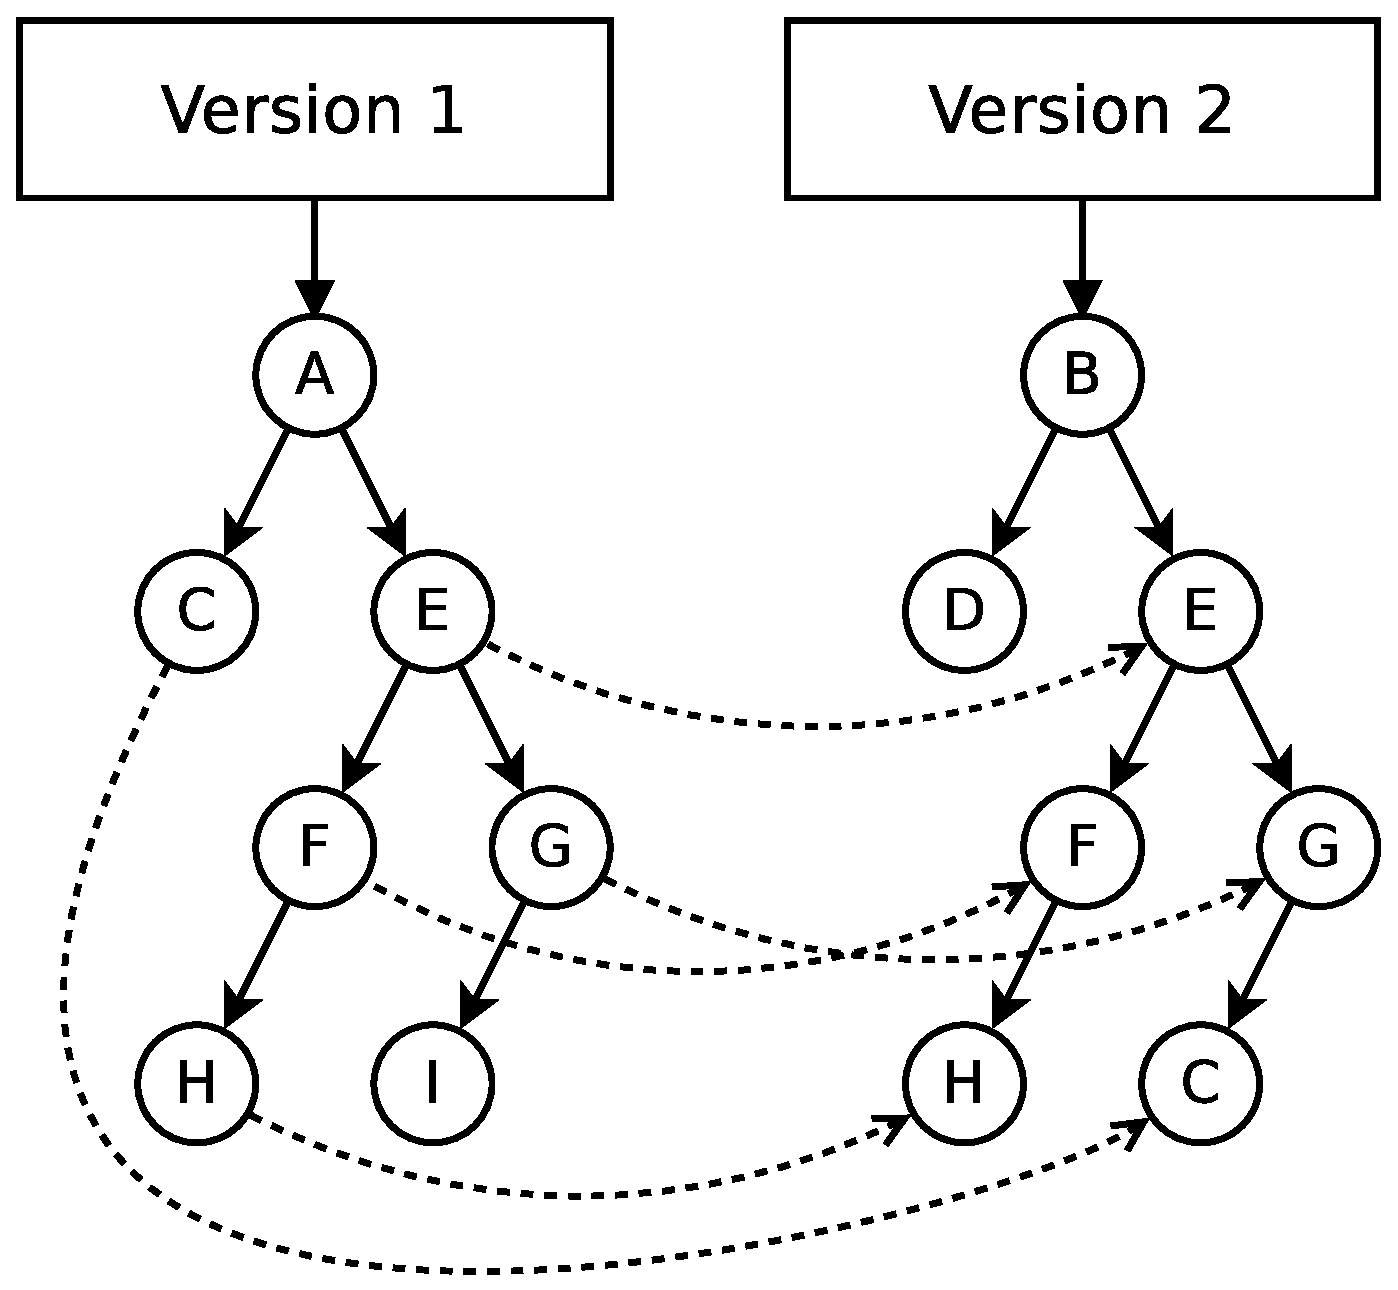
\includegraphics[width=0.66\textwidth]{figures/automatic_beh_inf/diagrams/dia2}
\par\end{centering}

\caption{Graphical representaton of tree mapping\label{fig:tree-mapping-example}}
\end{figure}



\subsection{Cluster construction}

Cluster construction comprises the grouping of nodes in subtrees,
and the readjustment of frontiers. Readjustment of frontiers is achieved
through the resizing of the clusters.


\subsubsection{Creating common subtrees}

At this point we have a mapping between the common nodes of both the
ASTs of the input modules. We now traverse the AST of one of the input
modules and, we group in subtrees the pairs of contiguous nodes that
have a mapping. That is, we find those groups of mapped nodes that
are contiguous in both trees and the mapping.

A pair of nodes $a$ and $b$ in a tree, (parent and child respectively),
are contiguous if and only if: the parent of the projection of $b$
is identical to the projection of $a$, and $b$ is child of $a$
in the same position, (same number of child), than the projection
of $b$ is child of the projection of $a$.

Formally, we have two sets of nodes $N$ and $M$, (one per AST of
input module, where $a,b\in N$), a function $f$ that maps pairs
of common nodes from $N$ to $M$ ($f:N\rightarrow M$), (as returned
by the tree matching algorithm in Section~\ref{sub:tree-matching}),
and functions $p$ and $q$, that map a node to a tuple with its parent
(inside the same AST) and the ordinal position of the node in the
list of children of its parent, ($p:N\rightarrow(N,\mathbb{N})$ and
$q:M\rightarrow(M,\mathbb{N})$). Two nodes $a$ and $b$ are contiguous
if and only if: $\exists(i\in\text{\ensuremath{\mathbb{N}})}:(a,i)=p(b)\land(f(a),i)=q(f(b))$,
or $\exists(i\in\text{\ensuremath{\mathbb{N}})}:(b,i)=p(b)\land(f(a),i)=q(f(b))$,
or if there exists a node $c$ that is contiguous to both $a$ and
$b$.

In Figure~\ref{fig:tree-clustering-example} we show how the trees
in Figure~\ref{fig:tree-mapping-example} would be clustered.

\begin{figure}
\begin{centering}
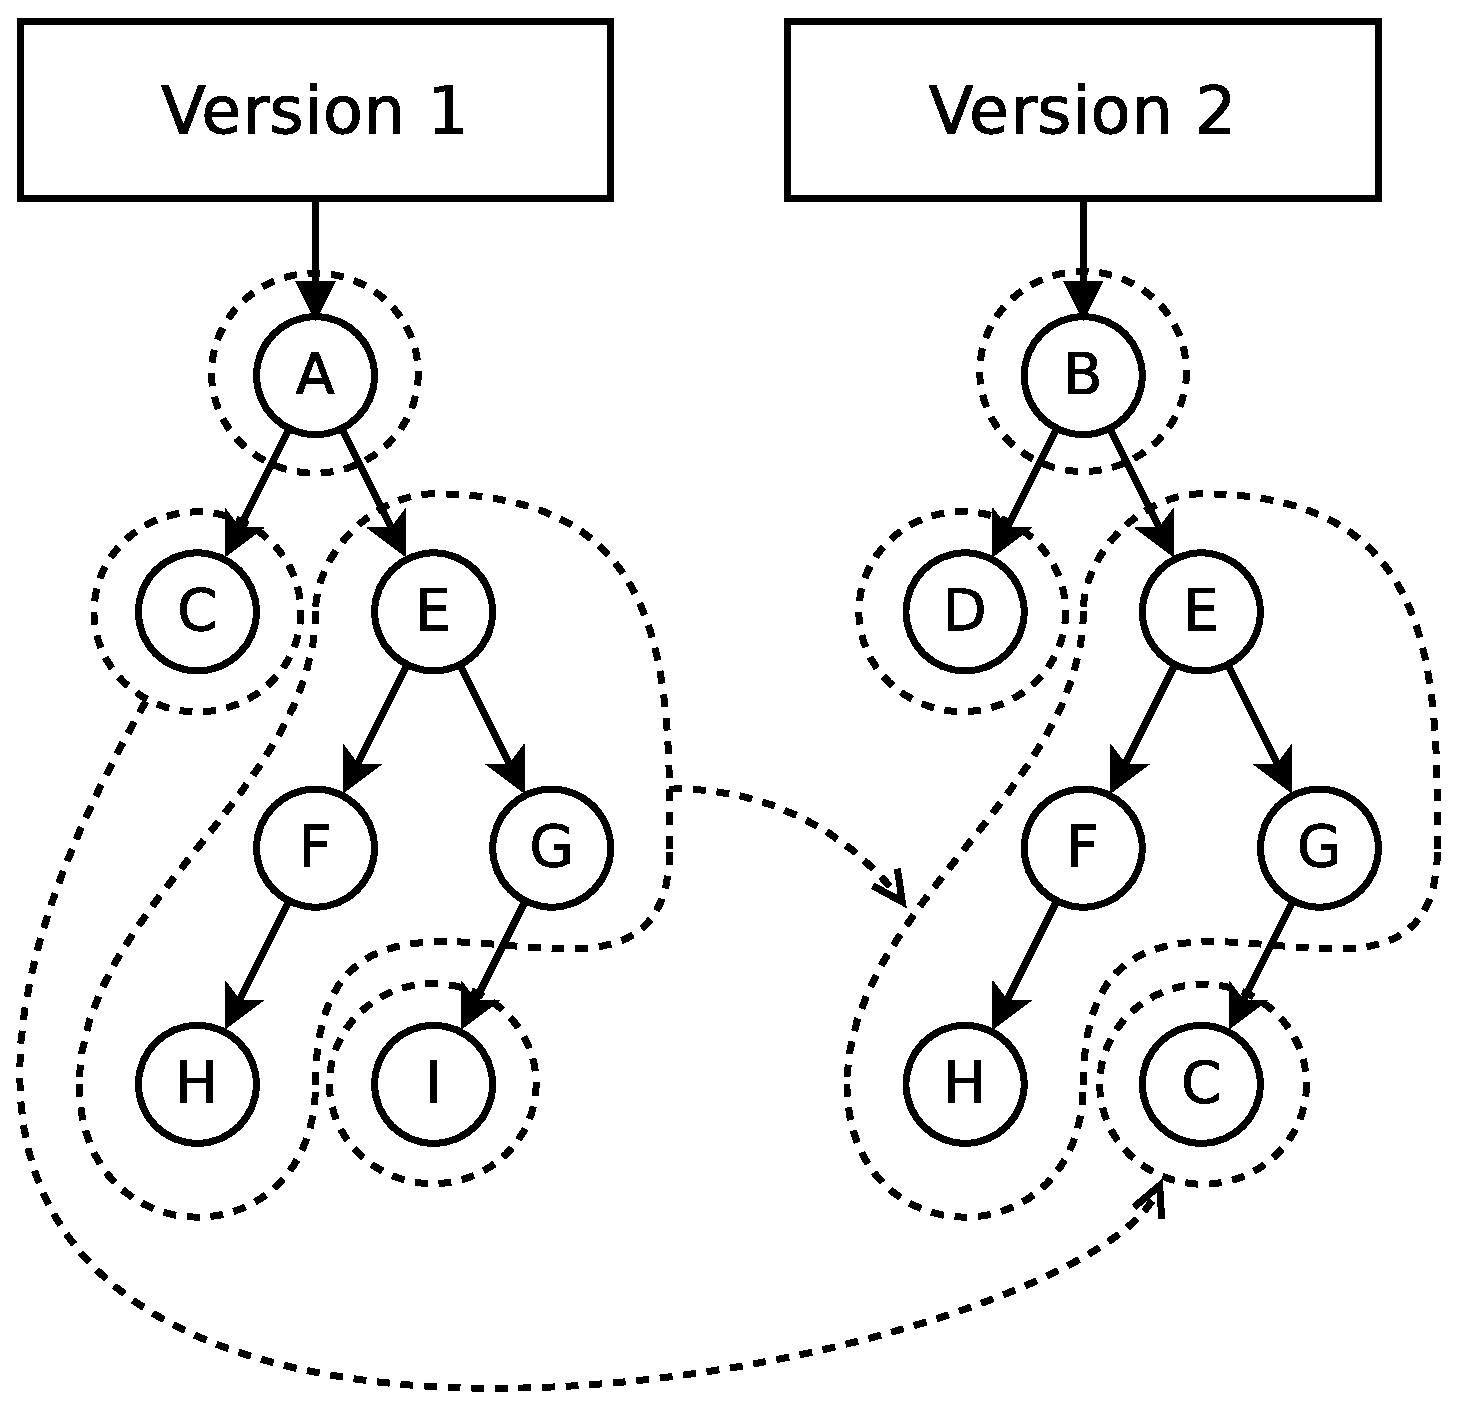
\includegraphics[width=0.69\textwidth]{figures/automatic_beh_inf/diagrams/dia3}
\par\end{centering}

\caption{Graphical representation of tree clustering\label{fig:tree-clustering-example}}
\end{figure}



\subsubsection{Readjusting the frontiers}

Once we have grouped all mappings in clusters, (i.e: contiguous subtrees),
we must check that the frontiers, (i.e: the pairs of parent-child
nodes with nodes in different clusters), are valid places for function
extraction. There are several reasons why this may not be the case,
the most common ones are:
\begin{itemize}
\item The lower node of the frontier must be an expression. In particular,
it must be syntactically correct to use the subtree of the frontier
as the body of a function.
\item It must be possible to replace the child node with a function call.
For example, a function call cannot be introduced in the header of
a function instead of a parameter.
\item The variables defined in the child subtree cannot be used outside
of it since creating a function will also create a new scope. This
can be allowed at this point and fixed afterwards in some cases.
\end{itemize}
The conditions for readjusting frontiers are also useful for fine
tuning the algorithm. We can allow the creation of invalid functions
as long as we have a postprocessing mechanism that fixes them, (see
Section~\ref{sub:function-migration-artifact}), and we can disallow
the creation of functions that would be correct, if we want to preserve
some artifacts or for readability (see
Section~\ref{sub:artificial-block-expressions}).

We can adjust the frontiers by removing pairs of nodes from the common
clusters, and by removing their mappings. This produces a small replication
of code, but in the worst case scenario, we will fallback to having
no common clusters and that would leave the input modules as they
were originally.

We take as basic principle that, if necessary, we can have code common
to both instances replicated in both the behaviour instances, but
we cannot have code exclusive to one of the behaviour instances in
the behaviour definition. We could potentially do so by adding conditional
flow control expressions, but that would prevent future generalisation,
(the creation of new instances for the generated behaviour definition).


\subsubsection{Common clusters and exclusive clusters}

After we have computed the nodes that will form the clusters, we group
the nodes that are not mapped (and, as such, do not belong to any
cluster), into exclusive clusters. We will still only group contiguous
nodes in each cluster, but this time we will consider two nodes are
contiguous if and only if:
\begin{itemize}
\item One is ancestor of the other for any of the ASTs of the input modules
\item None of the nodes that link them together, (in the AST hierarchy),
has a mapping with a noose in the other AST, (i.e: it does not belong
to a common cluster).
\end{itemize}
We will now have two kinds of cluster:
\begin{itemize}
\item The common clusters, that have representation in both ASTs. Each of
them represents a function in the output behaviour definition (or
common functions).
\item The exclusive clusters, that in turn belong to one of the two ASTs.
Each of them represents a function in one of the behaviour instances
(or callbacks).
\end{itemize}
In Figure~\ref{fig:cluster-linking-example}, we show how the example
in Figure~\ref{fig:tree-clustering-example} would be reorganised
and linked, where the dashed node I in Version 2 is the rendering
of an indirection cluster.

\begin{figure}
\begin{centering}
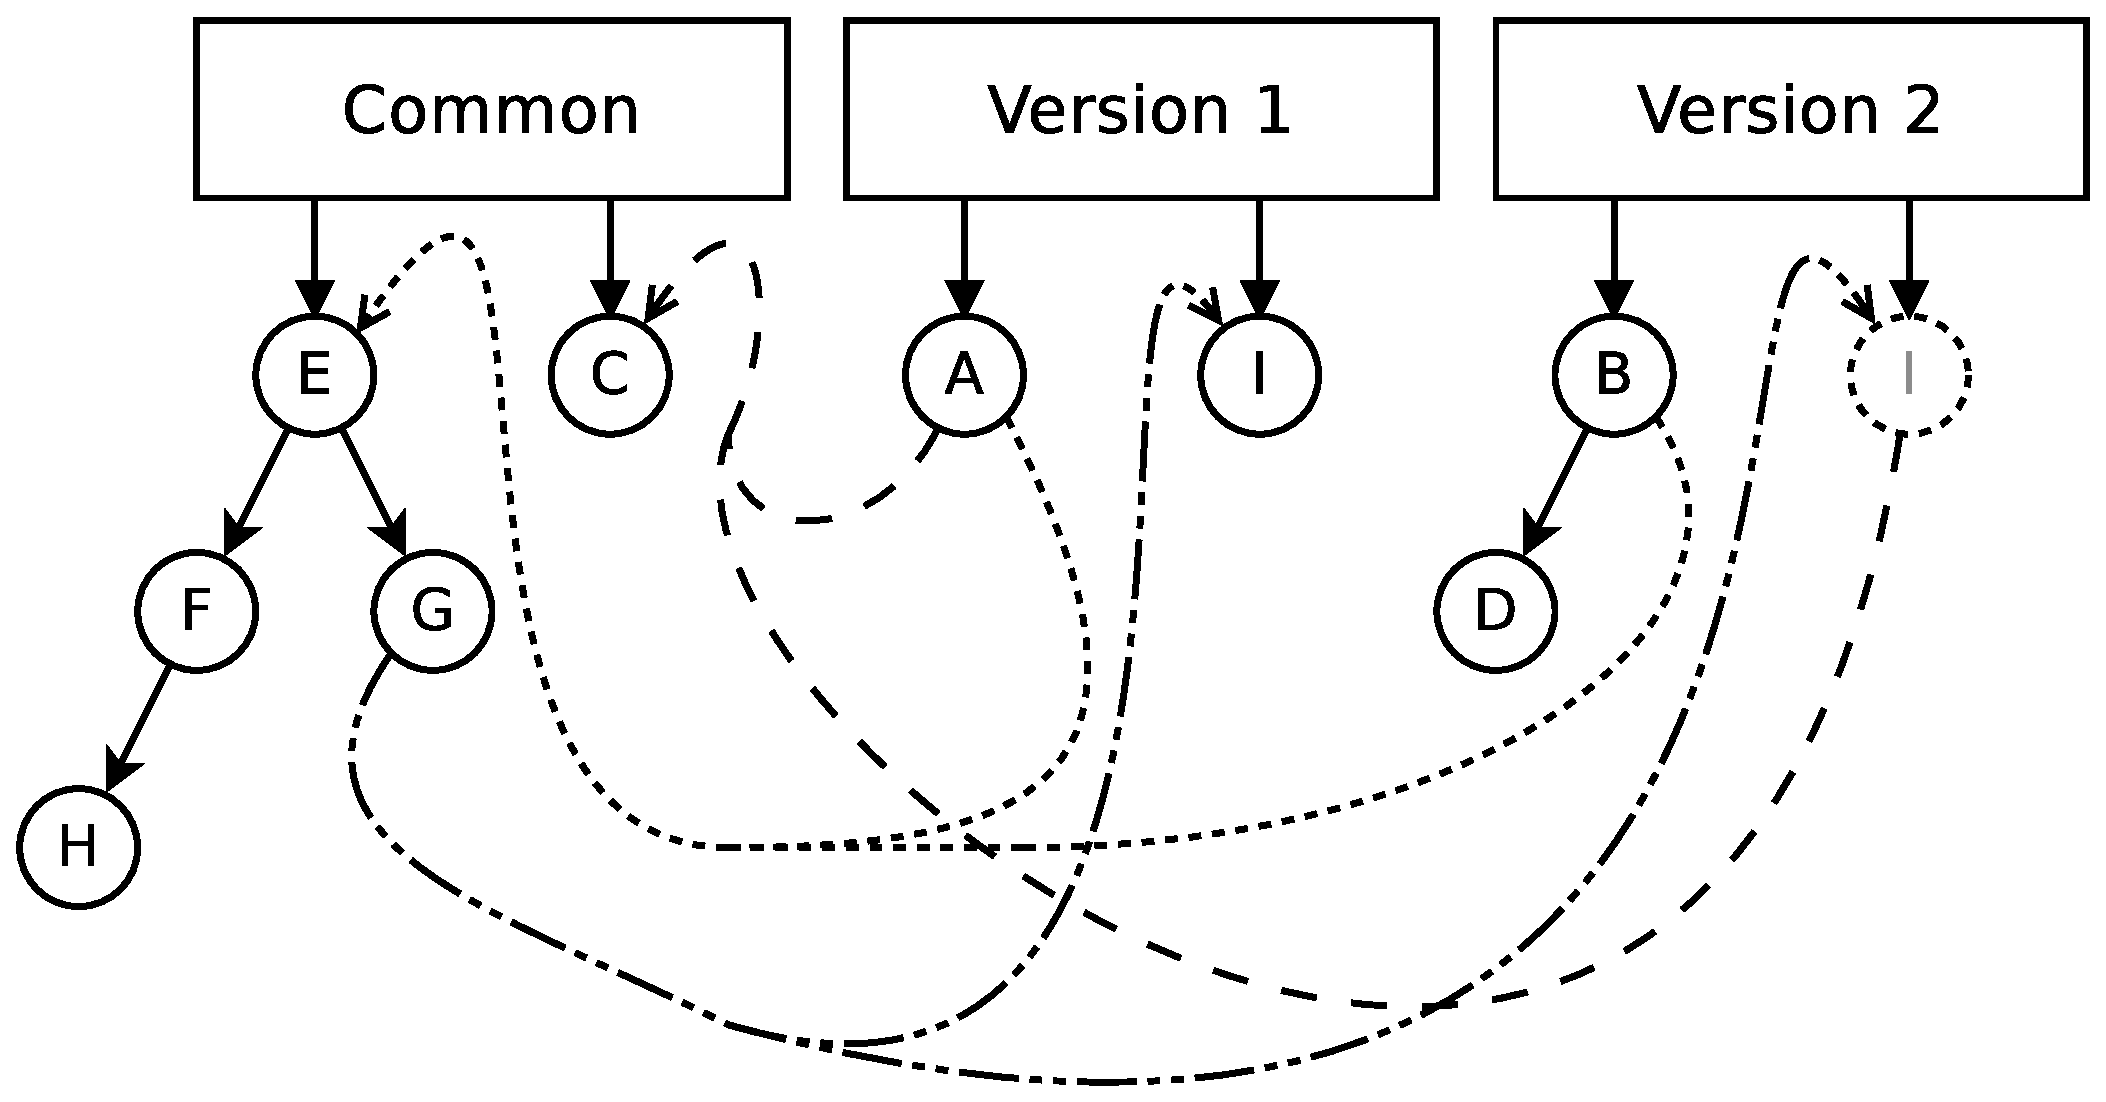
\includegraphics[width=1\textwidth]{figures/automatic_beh_inf/diagrams/dia5}
\par\end{centering}

\caption{Graphical representation of linking\label{fig:cluster-linking-example}}


\end{figure}



\subsection{Linking}

The last step is linking the clusters through function calls, to preserve
the behaviour of the original modules after the relocation of the
functions.

For linking, we first visit every lower frontier of common clusters,
and try to assign the same name to both alternative child clusters.
For each lower frontier in the common clusters we necessarily have
two alternative child clusters, since nodes in the common clusters
are the result of merging two nodes. We also know that these two clusters
are different, since otherwise they would have merged to the parent
cluster. We can find which clusters are these by looking up the original
nodes in both of the original ASTs.

The alternative child clusters for a lower frontier do not need to
be exclusive. It is possible that one or both of the child clusters
are also common. This is because the end of the cluster may be due
to a discontinuity rather than to exclusive behaviours. If that is
the case, it is also possible that we have already set a name for
those clusters.

In order to create a uniform interface, we need to keep the symmetry
in both behaviour instances. This means having the same number of
callbacks in both instances, and having the same number of arguments
for each pair of equivalent callbacks.

Because of this, if we have already set a name for the cluster and,
thus, we cannot ensure that both child clusters have the same name,
we will create exclusive ``indirection clusters'' in any or both
of the sides that cannot be renamed. Indirection clusters have, as
only body, a call that redirects the execution flow to the correct
child cluster. Of course, we want to minimise the use of indirection
clusters, since they add complexity to the code.

We can keep the number of parameters for equivalent callbacks equal,
by mixing the parameters of both alternatives at any point. If there
are common parameters, we add them only once, but we will add exclusive
parameters to both alternatives of each cluster. In the exclusive
side where the exclusive parameters of the opposite side are not bound,
we will use dummy values for those parameters. These dummy values
will not cause a difference in the behaviour because they will not
be used, and they are easy to generate thanks to the flexible typing
of Erlang.

\subsection{Extra considerations}

The automatic behaviour extraction refactoring implies several logical
subrefactorings, and, thus, some considerations applied to these subrefactorings
are also applicable to automatic behaviour extraction. The main logical
subrefactorings implied by automatic behaviour extraction are: function
extraction, and function module migration, (i.e: moving one function
from one module to another).

But, of course, there are some considerations that are specific to
this refactoring as well.

\subsubsection{Artificial block expressions\label{sub:artificial-block-expressions}}

As we have mentioned before, when encapsulating code into functions,
we must ensure that the created functions are valid, and that it is
syntactically and grammatically correct to insert a function call
in the position where the extracted code originally was.

Additionally, it is desirable that when several consecutive sentences
are extracted, they are combined into the same created function. This
is not trivial if, as in our implementation, the clusters created
have tree topology. Splitting a tree horizontally will create several
subtrees, which would in turn translate into separate functions. But
it is much clearer to have them grouped in the body of the same function,
rather than in several different functions which are called consecutively,
(e. g: without the block artifact, the input example modules in Figure~\ref{fig:block-expression-input},
would be merged as shown in Figure~\ref{fig:block-expression-before},
the block artifact allows the more concise representation shown in
Figure~\ref{fig:block-expression-after}).

\begin{figure}
\begin{minipage}[t]{0.5\columnwidth}%
\lstinputlisting[breaklines=true,frame=tbl,language=Erlang]{figures/automatic_beh_inf/1-block_artifact/1-in/mod1.erl}%
\end{minipage}%
\begin{minipage}[t]{0.5\columnwidth}%
\lstinputlisting[breaklines=true,frame=tblr,language=Erlang]{figures/automatic_beh_inf/1-block_artifact/1-in/mod2.erl}%
\end{minipage}

\caption{Input example modules to illustrate block expression artifact\label{fig:block-expression-input}}


\end{figure}


\begin{figure}
\begin{minipage}[t]{0.5\columnwidth}%
\lstinputlisting[breaklines=true,frame=tbl,language=Erlang]{
figures/automatic_beh_inf/1-block_artifact/2-out-before/mod1.erl}%
\end{minipage}%
\begin{minipage}[t]{0.5\columnwidth}%
\lstinputlisting[breaklines=true,frame=tblr,language=Erlang]{
figures/automatic_beh_inf/1-block_artifact/2-out-before/mod2.erl}%
\end{minipage}

\begin{minipage}[t]{1\columnwidth}%
\lstinputlisting[breaklines=true,frame=tblr,language=Erlang]{
figures/automatic_beh_inf/1-block_artifact/2-out-before/out.erl}%
\end{minipage}

\caption{Output of modules in Figure~\ref{fig:block-expression-input} without
block expression artifact\label{fig:block-expression-before}}
\end{figure}


\begin{figure}
\begin{minipage}[t]{0.5\columnwidth}%
\lstinputlisting[breaklines=true,frame=tbl,language=Erlang]{
figures/automatic_beh_inf/1-block_artifact/3-out-after/mod1.erl}%
\end{minipage}%
\begin{minipage}[t]{0.5\columnwidth}%
\lstinputlisting[breaklines=true,frame=tblr,language=Erlang]{
figures/automatic_beh_inf/1-block_artifact/3-out-after/mod2.erl}%
\end{minipage}

\begin{minipage}[t]{1\columnwidth}%
\lstinputlisting[breaklines=true,frame=tblr,language=Erlang]{
figures/automatic_beh_inf/1-block_artifact/3-out-after/out.erl}%
\end{minipage}

\caption{Output of modules in Figure~\ref{fig:block-expression-input} with
block expression artifact\label{fig:block-expression-after}}
\end{figure}


In our implementation we solve this problem by doing two passes to
the algorithm, after the first one, we locate the consecutive child
clusters and we introduce an artificial block expression around them,
(in both source modules). In the second pass, the blocks will be extracted
as a single function, and we can remove them easily at postprocessing.
We also ensure that artificial blocks are not detached from their
child sentences by adding an exception for them in the frontier readjustment
procedure.


\subsubsection{Exported variables}

Variables bound in a sentence of a function are accessible from the
following sequences of the function, even though they are located
at sibling subtrees. Because of that, if we extract part of a function
that defines variables used afterwards, we will move those variables
to a new scope, they will no longer accessible by the sibling trees,
and we will cause a compilation error.

This problem can be prevented by ensuring, when adjusting the cluster
frontiers, that there are no variables exported to the parent cluster.
But when combined with the artificial block expression artifact, this
would be interfering, by preventing the extraction of bigger blocks
which could be fixed to preserve the semantics just by adding some
small artifacts, (see Section~\ref{sub:interference}).


\subsubsection{Exported variables in artificial block expressions\label{sub:interference}}

We can export variables from a function extracted as a block if we
make it return a tuple with the variables exported and we match them
outside of the function call.

But in some cases the result of the function may already be used from
outside, and modifying it would modify the behaviour of the refactored
program. To avoid this, whenever variables are exported, we will only
create artificial block expressions that do not contain the last sequence
of a clause. We do not have to worry about modifying the value of
intermediate sentences in clauses, because we know that this values
were discarded in the original code, (e.g: in the code of Figure~,
we cannot extract a common function for the whole clause of the case
expression because it both exports and returns values, but we can
create one function for the last sentence and one for the rest as
shown in Figure~). This will not produce an ideal solution in every
case, and it is only implemented for when the frontier is in a clause,
but without it the previous approaches would modify behaviour in cases
where values are returned and exported simultaneously from a clause.

\begin{figure}
\begin{minipage}[t]{0.5\columnwidth}%
\lstinputlisting[breaklines=true,frame=tbl,language=Erlang]{figures/automatic_beh_inf/2-interference/1-in/mod1.erl}%
\end{minipage}%
\begin{minipage}[t]{0.5\columnwidth}%
\lstinputlisting[breaklines=true,frame=tblr,language=Erlang]{figures/automatic_beh_inf/2-interference/1-in/mod2.erl}%
\end{minipage}

\caption{Input example modules to illustrate interference between artifacts\label{fig:interference-input}}
\end{figure}


\begin{figure}
\begin{minipage}[t]{1\columnwidth}%
\lstinputlisting[breaklines=true,frame=tblr,language=Erlang]{figures/automatic_beh_inf/2-interference/2-out/mod1.erl}%
\end{minipage}

\begin{minipage}[t]{1\columnwidth}%
\lstinputlisting[breaklines=true,frame=tblr,language=Erlang]{figures/automatic_beh_inf/2-interference/2-out/mod2.erl}%
\end{minipage}

\begin{minipage}[t]{1\columnwidth}%
\lstinputlisting[breaklines=true,frame=tblr,language=Erlang]{figures/automatic_beh_inf/2-interference/2-out/out.erl}%
\end{minipage}

\caption{Output of modules in Figure~\ref{fig:interference-input}\label{fig:interference-output}}
\end{figure}


In the second pass we will ensure that there are no exported variables,
(apart from those in artificial block expressions), to avoid breaking
other unusual kind of frontiers where we cannot automatically fix
the exportation of variables, (e.g: match expressions in the elements
of a list). In those cases we will still keep the code consistency
in exchange for some replication.


\subsubsection{Module migration and dependencies}

Moving functions between modules also requires some considerations.
The behaviour of functions that must be moved may depend on the macros
used on the original module. Moving them without moving the macros
would alter their behaviour. These macros may define or import records,
external functions or macro definitions. In addition, these macros
may include conditionals, (i.e: \texttt{ifdef}, \texttt{ifndef}, \texttt{else},
and \texttt{endif}). There is no easy solution to combine the macros
of both modules that will work for every case. Because of this, we
opted for a compromise solution that will probably work for most cases,
we treat the outer conditional blocks of macros as single macros,
and we copy all the macros blocks that provide dependencies used in
the code that has been moved to the common module.

Another consideration to have when moving functions is to check that
none of the existing functions in the destination module conflicts
with the ones we are moving, in our case this is made easier by the
fact that the destination module is new and, as such, there are no
previous existing functions. Nevertheless, something similar can happen
for function whose name is not generated automatically (see Section~\ref{sub:function-arity-collision}).


\subsubsection{Function migration artifact\label{sub:function-migration-artifact}}

The headers of functions in Erlang, as in many languages, are hard to
divide through function extraction. Not being able to divide them
means that if two functions are very similar but they have slightly
different patterns, we are forced to keep the whole header of the
function in the exclusive modules and abstract only the body of each
of the clauses.

Nevertheless, if they are completely identical we can still generalise
them without modifying the interface. Even though we cannot insert
function calls on the root of a module, we can insert a very simplified
version of the interface of the function, move the whole function to the
common module, and insert a simple indirection.

We do this by accepting as a valid frontier the division between the
header of a function and the root of the module, and by artificially
detaching, (i.e: removing from the mapping and common cluster), the
root of the module.

During postprocessing, we just have to generate the simplified function
header around the function call that is left in the place where the
original function was, (example?).


\subsubsection{Function arity collision\label{sub:function-arity-collision}}

Functions created in the common module may, at some point, need to
call the exclusive modules back. The right exclusive module to call
is the one that called the current function in the first place. For
Erlang to know which module to call we parametrise the destination
module of the function calls in the common module with a variable,
passed as a parameter by the calling module. This variable will contain
the name of the module as an atom at any particular time, (example?).

The solution is simple, but adding a parameter to common functions
will still modify its arity. This is not a problem when the names
of the functions are generated and each function has a different name.
But if the function has been moved from the exclusive modules and
has a name assigned by the user, it may potentially clash with a different
function which has the same name but different arity.

It is necessary to have this in consideration, and rename one of the
clashing functions as soon as this happens, in order to avoid altering
the behaviour of the original code.



\section{Conclusions}
\label{concs}

The work reported here shows that we are able to automate the process of parametrising QuickCheck state machines -- that 
is extended finite-state machines -- in line with different versions or configurations of a system.



%\clearpage
\bibliographystyle{plain}
\bibliography{include/references}

\clearpage
\appendix
\section{This is an appendix}

\end{document}
